\documentclass[modern]{aastex62}

\usepackage{stix}
\usepackage{todonotes}
\newcommand{\vdag}{(v)^\dagger}
\newcommand\aastex{AAS\TeX}
\newcommand\latex{La\TeX}

\graphicspath{{./}{figures/}}
\shorttitle{HD106906b Time Resolved Observations}
\shortauthors{Zhou et al.}

\begin{document}


\title{HD106906 Working Papers}

\correspondingauthor{Yifan Zhou}
\email{yzhou@as.arizona.edu}

\author{Yifan Zhou}
\affil{Steward Observatory}

\begin{abstract}
  This documents keep the main result for \emph{Cloud Atlas} HD106906b \citep{Bailey2013} observations.
\end{abstract}

\keywords{}
\listoftodos

\section{Introduction}
HD106906b is a mid-L type planetary mass companion \citep{Bailey2013}.

\section{Observations}
The observations of HD106906 are part of HST large treasure program \emph{Cloud Atlas} (Program ID: 14241, PI: D. Apai). We used HST/WFC3/IR to observe HD106906 from 2016-01-29 20:45 to 2016-01-29 23:02 UTC for two consecutive HST orbits as part of the program variability amplitude assessment survey (VAAS). We then used the same instrument to observe the target from 2018-06-07 02:14 to 2018-06-07 12:35 for seven consecutive HST orbits for deep look observations (DLO). Light curves in F127M ($\lambda_{\mathrm{pivot}}=1.274\micron$, $\mathrm{FWHM}=0.07$), F139M ($\lambda_{\mathrm{pivot}}=1.384\micron$, $\mathrm{FWHM}=0.07$) and F153M $\lambda_{\mathrm{pivot}}=1.533\micron$, $\mathrm{FWHM}=0.07$ filters were taken in both observations. Exposure times were 66.4 seconds for the F127M and F153M frames and 88.4 seconds for the F139M frames. Filters rotated for every two to three frames through the entire observation sequences. Consequently, the observations in three filters were effectively simultaneous. The filter selection facilitated our goal of comparing HD106906b's rotational modulation in (F139M) and out of (F127M, F153M) the 1.4 \micron water absorption band.

Primary star subtraction is required for precision photometry of HD106906b because of the moderate contrast between the companion and its host star. The observation was set to enable two-roll differential imaging that could effectively subtract the point spread function (PSF) of the primary star. Between every two adjacent HST orbits, the position angle of the telescope differed by 31 degrees.  In this way the position angle of the companion to the host star in the image reference frame had the same difference between images from two orbits (Figure \todo{add figure}). Image subtraction removed the PSF structures that were associated with the telescope optical assembly but conserved the astrophysical signal, which primarily was HD106906b's PSF.

In total, we obtained 19 frames for each filter in the VAAS observation and 63 frames for each filter in the DLO observation. The photometric signal-to-noise ratio (SNR) for HD106906b was $\sim100$ per frame.

\section{Data Reductions}
% \subsection{Time-resolved photometry}

\begin{figure}
  \centering
  \plotone{figures/F127M_subtraction}
  \caption{Two-roll differential imaging result. }
  \label{fig:2rdi}
\end{figure}

Time-resolved photometry for HD106906b started with \texttt{flt} frames produced by CALWFC3. This data reduction component included four steps: image preparation, primary star subtraction, PSF fitting photometry, and light curve systematics removal.

Image preparation sorted \texttt{flt} frames into data cubes for subsequent image processing. Before place images into data cubes, we first made bad pixel mask and remove sky background for every frame. Pixels that have data quality flags 4 (bad detector pixel), 16 (hot pixel), 32(unstable response), and 256 (full-well saturation) were identified as ``bad pixels'' and excluded from subsequent analyses. After masking out pixels with those data quality flags, we examined the imaged by eye to identify and mask remaining spurious pixels. To remove sky background, we first drew circular masks around all visible point sources in the field and then applied a five-iteration sigma-clip to further exclude bright pixels. The median value of the unmasked pixel was the sky background and  removed from the images. The background removed images as well as the associated bad pixel masks were sorted by time and  formed the data cube.

We then applies two-roll differential imaging (2RDI) to subtract the PSF of HD106906AB. First, we registered the images by the centroid of HD106906AB. The centroid coordinates of HD106906AB were measured relative to those of the first image frame using two-dimensional cross-correlation and further refined by residual least $\chi^{2}$ minimization in the diffraction spider region. We then selected best PSF image from candidate PSF image. Every image that was taken with different telescope roll angles as the target image was a candidate PSF. The candidate PSF was linearly scaled to minimize the least squared residual in an annulus around HD106906AB (Figure \ref{fig:2rdi} \todo{Show the optimization region}), and the best PSF was the one that has the smallest residuals. Finally, we subtract the best PSFs from original images and obtained primary subtracted images (Figure \ref{fig:2rdi}). 

HD106906b's photometry was measured by PSF fitting to the primary subtracted images. We construct $9\times$ over-sampled PSFs using TINYTIM. Free parameters for the model PSFs were the centroid coordinates, HST secondary mirror displacement, and the scale of the PSF. We optimized these parameters by $\chi^{2}$ minimization, which was performed by Markov Chain Monte Carlos. We normalized the total flux for the model PSF with an infinite large radius. Therefore the best fit scale of the PSF was the total flux  of HD106906b with that includes aperture correction. We use the World Coordinate System information that are in the fits file header to convert the centroid coordinates to RA and DEC astrometry.

The uncertainties of light curves in F127M, F139M, and F153M are all dominated by random noise that includes photon noise, readout noise, and dark current. However, light curve analyses require systematic noise in the light curve to be accurately characterized and corrected. For WFC3/IR light curves, charge trapping related ramp effect is the major component of the systematic noise. We use RECTE \citep{Zhou2017} to model and remove the ramp effect systematics from the light curves. The ramp effect removal procedure follows \citet{Zhou2019} that details the application of RECTE in time-resolved direct imaging observations. We calculate ramp profiles by feeding the entire direct image time series into RECTE and forward-modeling the charge trapping processes. The model ramp profiles are then divided from the uncorrected light curves, which results in corrected light curves. 

\section{Results}
% \subsection{Image}
\subsection{Photometry, light curves and variability}

\newcommand{\fluxunit}{\ensuremath{\mathrm{ergs}\,\mathrm{cm^{-2}}\,\mathrm{s^{-1}}\,\mathrm{\micron^{{-1}}}}}
We obtained single frame photometry at SNRs of 77, 78, and 105 in the F127M, F139M, and F153M bands, respectively. After aperture correction, the absolute flux intensity in these three bands are $6.23\pm0.08\times10^{-13}\fluxunit$, $3.71\pm0.05\times10^{-13}\fluxunit$, and $4.35\pm0.04\times10^{{-13}}\fluxunit$, respectively. The flux uncertainty are for average $1-\sigma$ uncertainty in a single frame. Figure~\ref{fig:lightcurve} shows the corrected and normalized light curve in the F127M, F139M, and F153M bands.  No large amplitude ($>1\%$) rotational modulations are identifiable in all three light curves. Variations in the light curve are dominated by random noise whose major component is photon noise. Comparing to flat lines, the three light curves have reduced-$\chi^{2}$ of 1.89, 1.47, and 1.1 for the F127M, F139M, and F153M bands, respectively.

To investigate light curve periodicity, we derived the power spectra for the light curves using Lomb-Scargle periodogram method \citep[][Figure~\ref{fig:periodogram}]{Lomb1976}. The power spectra for the F139M and F153M light curves do not have any significant peaks except in the high frequency ends of the power spectra, which are dominated by random noise. The lack of structures in the F139M and F153M power spectra is consistent with the featureless light curves. The power spectra for the F127M light curve does clearly peaks at 4.02 hr. Fitting a single 4.02 hr sine wave to the F127M light curve marginally decreases the reduced-$\chi^{2}$ from 1.89 (for a flat line) to 1.53. The best-fitting parameters of the 4.02 hr sine wave are $\mathrm{amplitude}=0.49\pm0.12\%$, $\mathrm{phase} = -1.57\pm0.29$ rad. Figure~\ref{fig:fold} shows the F127M light curve folded to the 4.02 hr period.

In summary, HD106906b shows marginal evidence of variability in the F127M band, which is the bluest band in the observations. Light curves in the other two bands (water absorption, red side of water band continuum) are consistent with flat lines.

\begin{figure}
  \centering
  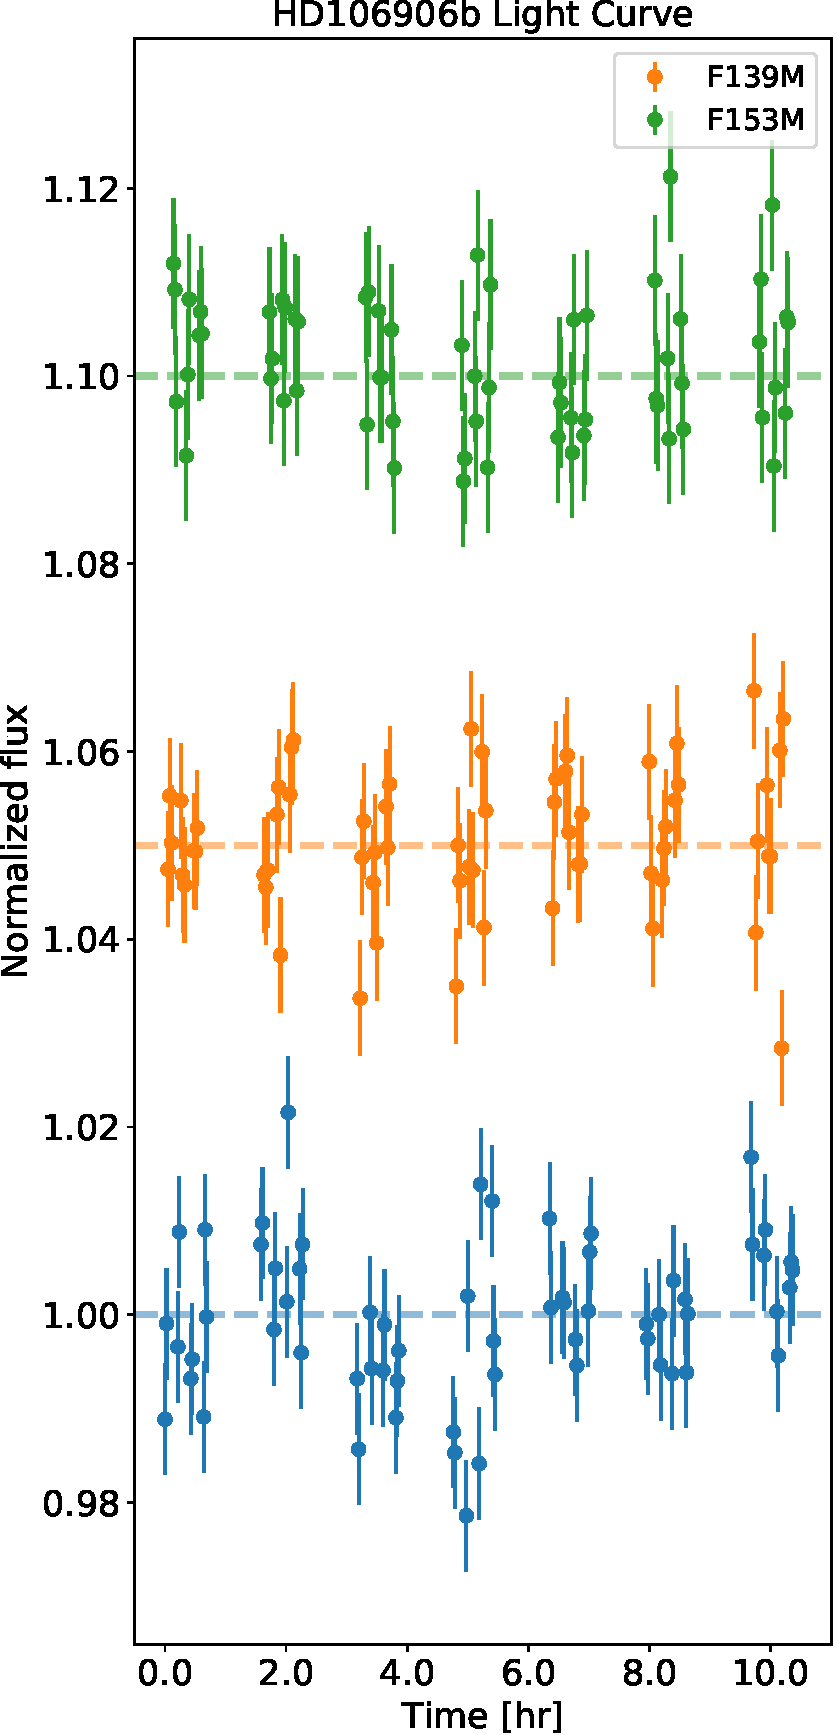
\includegraphics[width=0.5\textwidth]{figures/HD106906_lightcurves.pdf}
  \caption{The light curve for HD106906b in the F127M, F139M, and F153M}
  \label{fig:lightcurve}
\end{figure}

\begin{figure}
  \centering
  \plotone{figures/HD106906_powerspectrum.pdf}
  \caption{Lomb-Scargle periodogram for the light curves of HD106906b.}
  \label{fig:periodogram}
\end{figure}

\begin{figure}
  \centering
  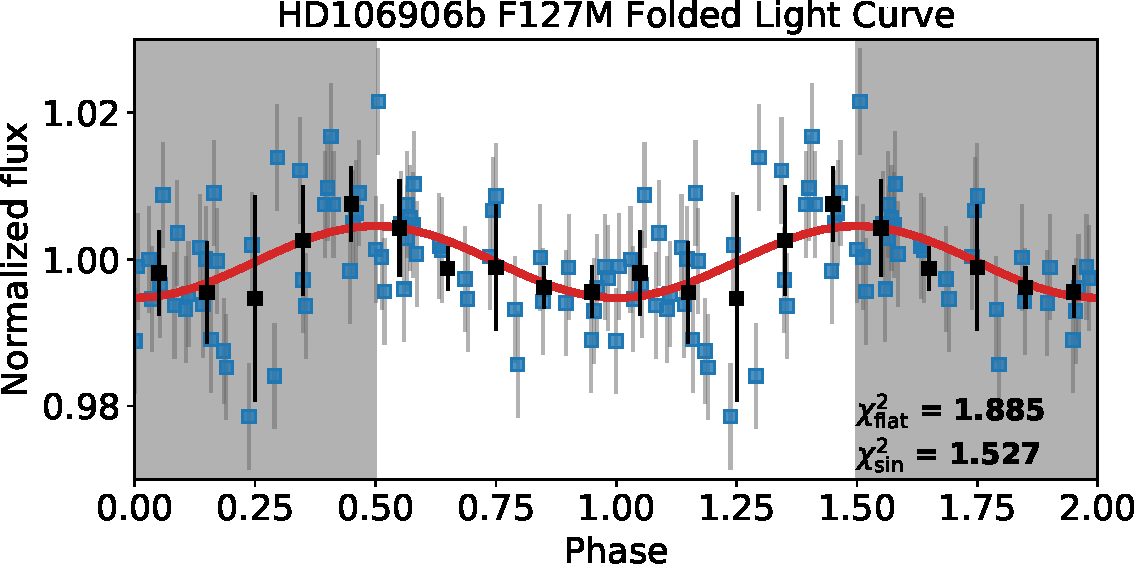
\includegraphics[width=0.5\textwidth]{figures/F127M_foldedLC.pdf}
  \caption{Phase-folded light curve for F127M. The light curve is folded to a period of 4.02 hr. The period corresponds to the most significant peak in the Lomb Scargle periodogram.}
  \label{fig:fold}
\end{figure}

\subsection{Modulation significance evaluation}

We evaluate the modulation significance in both instrumental and astrophysical perspective. From the instrumental point of view, we have two arguments against that the modulation signal we see in HD106906b's F127M light curve is due to systematics. First, the F127M, F139M, and F153M observations were taken \emph{de facto} simultaneously. Systematics that introduces periodic/sinusoidal signals at 4 hr timescale in the F127M light curve should have similar effect on the other two light curves. Agreement between F139M and F153M light curves with flat lines is inconsistent with modulation in the F127M light curve being systematics. Second, similar modulations do not appear in the light curves of background stars. We measure and analysis light curves of fifteen brightest background stars that are in the field of view of both telescope roll angles and are not affected by the diffraction spikes of the primary PSFs. In the appendix we list the light curves and periodograms for all background stars. Figure \ref{fig:all-periodograms} shows the comparison between the periodograms of the background stars and that for F127M light curve of HD106906b. Most periodogram of the background star do not show significant signals except one object. However, when we fold its light curve to the period with the most significant peak, the folded light curve is consistent with a flat line. These two lines of evidence argue that systematics is not likely to be the cause of the modulation signal.

From astrophysical perspective, we evaluate the likelihood for HD106906b to be rotationally modulated only in the F127M band but not the other two bands. Multi-wavelength and time-resolved observations of ultra-cool dwarfs have found the rotational modulations for majority  brown dwarfs and planetary mass companions are spectrally dependent and have greater amplitude at shorter wavelengths than longer wavelengths \citep[e.g.,][]{Zhou2019,Zhou2016,Yang2014,Apai2013,Schlawin}. This phenomenon is consistent with theoretical estimation based on Mie-scattering calculation\citep{Schlawin,Hiranaka2016}. In addition, the 1.4 \micron{} water absorption/F139M band often show damped rotational modulation, due to water vapor opacity elevating the photosphere at this wavelength.  Therefore rotational modulation only appearing in the bluest band of our observation is qualitatively consistent with theoretical model and previous observations, particularly those for planetary mass companions \citep{Zhou2016,Zhou2019}. If we assume that the wavelength dependence of HD106906b's rotational modulation is the same as that measured in 2M1207b \citep{Zhou2016}, as 2M1207b is the closest analogue that also has modulation detected, a 0.49\% modulation in the F127M band should correspond to a 0.06\% modulation in the F153M band. Such a small amplitude is below the sensitivity of our observation. Therefore, if the overall modulation amplitude is small, it is likely that the signal is only detected in the bluest band of the observation.

These two lines of evidence support the modulation we see in HD106906b's F127M light curve to be astrophysical origin, in particular, caused by heterogeneous clouds. Nevertheless, we emphasize that the amplitude of the signal is small and marginally detected. Our evaluation on the rotational modulation and rotation period for HD106906b remain inconclusive.

\begin{figure}
  \centering
    \plotone{figures/all-LSs}
  \caption{Comparison of the periodograms between those for background stars and those for HD106906b. The two background star periodograms that show simialr signals as HD109606b's do not show variations in the folded light curves.}
  \label{fig:all-periodograms}
\end{figure}


\subsection{Spectral Energy Distribution}
We combine our photometry results with archival data to investigate the spectral energy distribution (SED) of HD106906b.  We take HST/ACS/F606W band ($\lambda_{\mathrm{pivot}}=0.596\micron$, FWHM$=0.234\micron$) from \citet{Kalas2015}, $K_{s}$ ($\lambda_{\mathrm{pivot}}=2.145\micron$, FWHM$=0.305\micron$) and $L'$ ($\lambda_{\mathrm{pivot}}=3.774\micron$, FWHM$=0.592\micron$) bands from \citet{Bailey2013}. We do not use the archival $J$ band photometry because our F127M photometry characterizes similar spectral features and has more than $20\times$ greater SNR. Our F139M photometry provide a tight $1.4\micron$ water absorption constraint for HD106906b.

We fit the SED of HD106906b to the BT Settl \citep[][Figure~\ref{fig:SED}]{Allard2012}. We perform model fitting in magnitude scale, for which we convert the flux intensity to magnitude and linearly interpolate the model grid in magnitude scales. The free parameters are effective temperature $T_{\mathrm{eff}}$, surface gravity $\log g$, and a scaling parameter. Because the model SED is presented as the flux at the photosphere surface, with known distance the scaling parameter can be translate to the photospheric radius. Using least $\chi^{2}$ criterion, we result in best-fitting $T_{\mathrm{eff}}$ of $1,800\pm100$~K and $\log g=5.5\pm0.5$.  The scaling parameter corresponds to a radius of  $1.775pm0.015R_{\mathrm{Jup}}$ at a distance of 103.3~pc \citep{Gaia2018,Gaia2016}. The 1,800~K effective temperature estimate is consistent with previous study \citep{Bailey2013,Wu2016}, but the surface gravity is not compatible with a low surface gravity assessment. In addition, the model SED under-predicts the F139M band flux, or over-predicts the depth of the water absorption band.

\begin{figure*}
  \centering
  \plottwo{figures/SEDfit.pdf}{figures/SEDfit_zoomin.pdf}
  \caption{The SED of HD106906 and the best-fitting BT Settl model. The left panel shows the full observed SED (blue) that includes photometry from both this observation and archival data. The red line is the best-fitting BT Settl spectrum (1800~K, $\log g=5.5$). The red dots are the model photometry that are from model spectrum integrated with the filter throughput curves. The right panel zooms in the wavelength range of this observation. The orange violin plot shows the uncertainty of the model fitting. The flux in the F139M band is significantly under-predicted by the BT Settl model.}
  \label{fig:SED}
\end{figure*}

\subsection{Astrometry}
\label{sec:astrometry}
We are particularly interested in the background star that is only 0\arcsec{}.87 away from HD106906b, because it is unreported in previous studies and could contaminate the photometric and spectroscopic observations of HD106906b. We calculated the differences in right ascension ($\Delta$RA) and declination ($\Delta$DEC) and the separations between HD106906b and the background star from year 2003 (one year before the first direct imaging record of HD106906b) to year 2023. In this calculation, the background star is assumed to be stationary and HD106906b is co-moving with its host star at $(\mu_\alpha\cos\delta=-39.01 \mbox{mas/yr}, \mu_{\delta}=-12.87 \mbox{mas/yr})$ \citep{Gaia2016, Gaia2018}. The results are shown in Figure~\ref{fig:astrometry:bck}. In the same figures, we also marked the previous observations \citep{Bailey2013, Wu2016, Lagrange2016, Daemgen2017} to evaluate if the background star was detectable or could contaminate the measurements in those observations.

Figure~\ref{fig:astrometry:bck} demonstrates that HD106906b, due to its proper motion, has been approaching  the background star over the years. The separation between these two object has shortened from 1\arcsec.29 (2004, first imaging record) to 0\arcsec.87 (this study). In the study of \citep{Bailey2013, Wu2016, Daemgen2017}, the background star had separation of 0.95-1.05 to HD106906b. Given their separations in these studies, it is unclear if the background star contaminated those measurements. Considering the brightness contrast of the two object, in the worst case, the contamination of the background star to HD106906b's broadband photometry is  $<7.5\%$.

\begin{figure}
  \centering
  \plottwo{figures/bckStarDeltaRADEC.pdf}{figures/bckStarSeparation.pdf}
  \caption{Relative astrometry between HD106906b and a closeby background star. Left: The difference in right ascension and declination. Right: The separation as a function of time. Past observations of HD106906b are marked as squares.}
  \label{fig:astrometry:bck}
\end{figure}

\subsection{Other sources in the field}
Our $30\arcsec\times30\arcsec$ field of view (Figure \ref{fig:RGBimage}) is a crowded field that may include yet undiscovered companion of HD106906. The three filters that are used in this observation measure the water absorption depth, which is an effective criterion to select ultra-cool objects. Here we define the water absorption depth as the difference between the F139M flux intensity and the continuum, which is average flux intensity of F127M and F153M. This difference is further normalized by the continuum flux to get the relative water absorption depth. The relative water absorption depth is calculated as the following equation.
\begin{equation}
D = \frac{(f_{\mathrm{F127M}} + f_\mathrm{F153M})/2 - f_{\mathrm{F139M}}}{(f_{\mathrm{F127M}} + f_\mathrm{{F153M}})/2}
\end{equation}
We used the median combined primary subtracted image to measure the relative water absorption depth for 12 point sources (include HD106906b) that are in the field of view for both telescope rolls. Figure~\ref{fig:backgroundsources} shows the water absorption depth for each source. Except HD106906b, there is one source that has significant water absorption depth. Interestingly, this source is the one that is discussed in \S\ref{sec:astrometry}, and also the one that has the smallest angular separation to HD106906b among all sources in the field of view. However, based on the discussion of \S\ref{sec:astrometry}, this source is unlikely to be co-moving with HD106906. Its astrometry is consistent of being a background star.

\begin{figure}
  \centering
  \plottwo{figures/HD106906_RGB}{figures/HD106906_RGB_zoomin}  
  \caption{R (F153M) G (F139M) B (F127M) images of HD106906 (left) and the zoomed-in view of the planet. The PSF of the planet has less green shade compared to background stars due to strong water absorption of HD106906b.}
  \label{fig:RGBimage}
\end{figure}
\begin{figure}
  \centering
  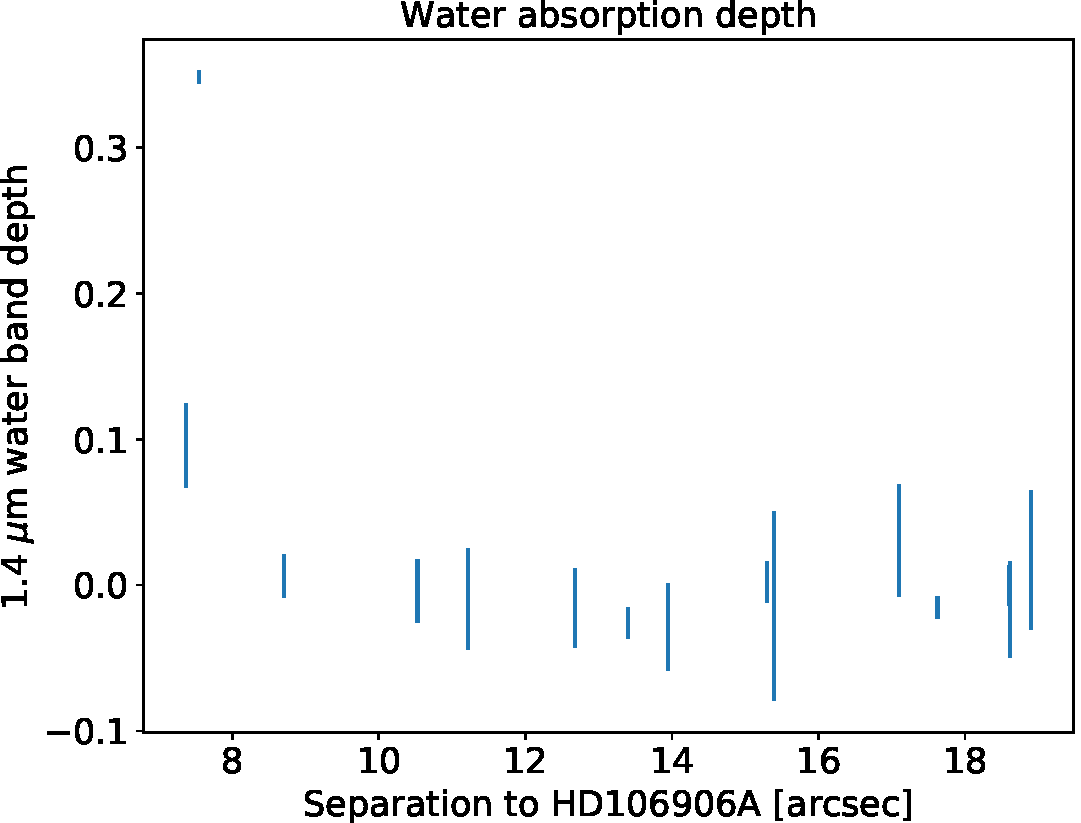
\includegraphics[width=0.5\textwidth]{figures/bck_waterdepth.pdf}
  \caption{Water absorption depths of all sources in the field of view. The sources are ranked by their angular distance to HD106906AB. The two sources (one is HD106906b) that have significant water absorption are also the two that are closest to HD106906AB in agnular distance.}
  \label{fig:backgroundsources}
\end{figure}

% \Interestingly{Large scale structures}


\section{Discussion}
\begin{enumerate}
\item variability:]\\
  color dependence, compare with other planetary mass companions
\item the limit on the inclination \citep[see][]{Vos2017}
  
\item SED of HD106906. Deviation from BT Settl model. The best-fitting $\log g$ is very high (5.5)
\item possible astrometry constrains (what about the distortion correction for WFC3)\\
\item limit on additional companions\\
  % \item lack of large amplitude detection for planetary mass companions.\\
%   depend on the analysis of the first step
\end{enumerate}

\subsection{SED of  HD106906b}
Two issues have emerged in the SED fitting results. First, the best-fitting model over-predicts the 1.4 \micron{} water absorption band depth. Second, the best-fitting surface gravity is inconsistent with previous low-gravity assessment for HD106906b.

To investigate the first issue, we calculate the water band absorption depths in the BT Settl as functions of $T_{\mathrm{eff}}$ and $\log g$ and compare them with the observed value. As shown in Figure \ref{fig:waterdepth}), for a fixed $T_{\mathrm{eff}}$ of 1800 K, all BT Settl models over-predict the water band depth. For a fixed $\log g$ of 5.5, to match the observed water band depth, $T_{\mathrm{eff}}$ needs to be raised to $2500$ K, although such a high temperature is not at all consistent with the overall SED shape. Therefore, the mismatch between the HD106906b's observed and the model SEDs in the 1.4 \micron{} water bands demonstrates the inadequacy of current state-of-the-art ultra-cool atmospheric models.

\citet{Bailey2013} and \citet{Daemgen2017} have discussed the surface gravity of HD106906b. Both studies classify HD106906b as a low-to-intermediate surface gravity object based on its triangle-shaped $H$ band spectrum. The equivalent widths of the K I absorption lines measured in \citet{Daemgen2017} are also consistent with an intermediate surface gravity classification. In addition, low surface gravity is also consistent with the young and low mass nature of HD106906b. However, our SED fitting yield a very high gravity result. With a fixed $T_{\mathrm{eff}}$ of 1800 K, lower surface gravity models significantly over-predicts the F153M and $K_{\mathrm{s}}$ band flux intensities, therefore they are not preferred by the SED fitting. This inconsistency, again, may show the insufficiency of atmospheric models for planetary-mass ultra-cool objects.

\begin{figure}
  \centering
  \plottwo{figures/logg_water}{figures/Teff_water}
  \caption{1.4 \micron{} water band depths predicted by the BT Settl model. Left: With a fixed $T_{\mathrm{eff}}=1800$ K, models with $\log g$ between 3 to 5.5 all over-predicts the water band depths. Right: With a fixed $\log g=5.5$, it requires $T_{\mathrm{eff}}=2500$ K for the model to match the observation.}
  \label{fig:waterdepth}
\end{figure}

% \end{enumerate}
% For the last point, take the variability occurrence rate from \citep{Vos2017,Metchev2015}, test whether the low mass companions' variability occurrence rate agree with the low surface gravity field objects
\bibliographystyle{yahapj}
\bibliography{library}

\end{document}
%%% Local Variables:
%%% mode: latex
%%% TeX-master: t
%%% End:

% LocalWords:  AAS
